\section{Spectrum by Accretion of Matter}
\label{sec_accretion}
\begin{quotation}
	\raggedleft \it
	Simulations are like miniskirts,\\
	they show a lot, but hide the essentials.\\
	-- Hubert Kirrmann
\end{quotation}
The observed spectrum of the object at the centre of our galaxy is quite unusual. The spectrum seems to have no emission in the infra-red (IR)
region, due to a very steep `cut-out' between $10^{12}$ and $10^{13}$Hz \cite{ref_meliareview}.
In this section, we investigate a very simple Newtonian accretion model \cite{ref_FKR},
which assumes that the accretion disk is both geometrically thin and optically thick (we will return to the non-validity of this assumption
later). We will show how a mass distribution, such as that of a fermion ball, will naturally produce this sudden drop in the accretion
spectrum.

\subsection{Source of the Accreting Gas}
Radio continuum observations have revealed a `cometary tail' of ionised gas from IRS7 (the brightest 2$\mu$m source in the central
parsec of the galaxy) leading away from the the location of Sgr A*. The tail appears to be formed by a `circumnuclear' wind which has been
observed originating from the cluster of stars IRS16 (which is an IR source close to, but not incident with Sgr A*) \cite{ref_yusefmorris}.
This collision is highly supersonic and creates a bow-shock within the gas flows \cite{ref_melia}, see Figure \ref{fig_irs7}.
This bow-shock dissipates most of the directed kinetic energy and heats the gas to $7 \times 10^6$K.

\begin{figure}[p]
	\begin{center}
	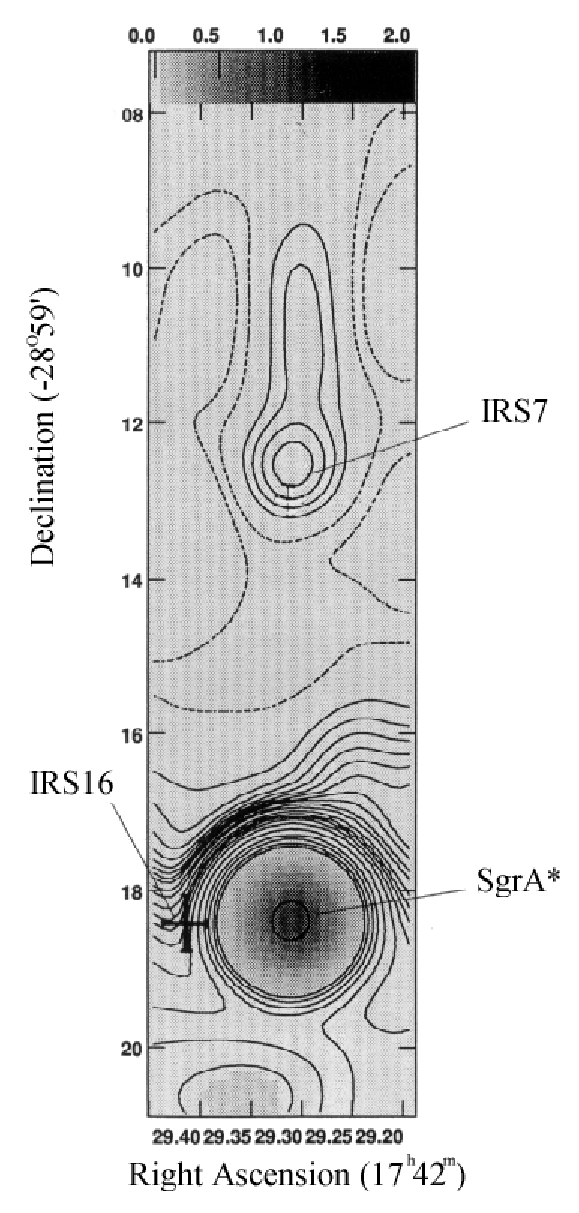
\includegraphics[angle=0,width=0.4\textwidth]{eps/irs7.eps}
	\caption{Contour map at $\lambda=2$cm of the IRS7 `cometary tail' with relation to Sgr A*. The tail is a result of the collision between
	the galactic centre and stellar winds rather than from the motion of IRS7 through the interstellar medium \cite{ref_yusefmorris}.}
	\label{fig_irs7}
	\end{center}
\end{figure}

Assuming that Sgr A* is not itself the source of the gaseous outflow, we may treat this gas as an excellent candidate for accretion
`fuel' in powering the spectrum, observed from the central object. We assume the shocked plasma falls in radially toward the central
object and that the accretion begins at radius $R_a$, given by the escape velocity
\begin{equation}
	R_a=\frac{2GM}{v_{gw}^2}
	\label{eqn_accretionstartradius}
\end{equation}
where $v_{gw}= 500 \rightarrow 700$ km/s. By simply comparing this velocity with Figure \ref{fig_escapevelocities}, we see that $R_a$
is significantly outside the fermion ball such that this equation will result the same for both scenarios. Although the limits of
accretion rate ($\dot{M}$) have been estimated in \cite{ref_melia} as $3 \rightarrow 40$ $\times 10^{-3}M_\odot$/yr,
is is widely accepted that the true values are much lower. The system
is therefore much below the Eddington-limited accretion rate and is called `weakly accreting'.
%\textcolor{red}{[I personally don't believe it is `much' below the Eddington-limited accretion rate!]}
We also take the most probable inclination angle of the accretion disk as $60^\circ$.

\subsection{Viscous Torque as a Means of Energy Release}
Consider 2 shearing `rings' in a gas of width $\lambda$, which meet at a surface of (radial) position $R$. Due to chaotic motions, gas
elements are constantly exchanged across this surface with speeds $\simeq \tilde v$. A typical element travels a distance $\lambda$ before
interacting on the other side of the surface.

These elements of fluid carry slightly different amounts of angular momentum, corresponding
to their location, either $R - \frac{\lambda}{2}$ or $R + \frac{\lambda}{2}$ (the substitutions $R_- = R - \frac{\lambda}{2}$ and
$R_+ = R + \frac{\lambda}{2}$ are made for clarity). This process cannot result in any net transfer of matter between the rings as
it occurs in equilibrium, therefore mass crosses the surface at equal rates in both directions of the order $\xi \widetilde{v}$ per unit
arc length, where $\xi$ is the surface density.

As the elements each possess separate angular momenta, there is a net transfer due to the chaotic processes, a `viscous torque' exerted
on the outer stream by the inner, et vice versa. The fluid at $R - \frac{\lambda}{2}$ will appear (to an observer moving with the rings)
to have velocity
\begin{equation}
	R_- \Omega (R_-) - R \Omega(R)
	\label{eqn_fluidvelocity1}
\end{equation}
and at $R + \frac{\lambda}{2}$
\begin{equation}
	R_+ \Omega (R_+) - R \Omega(R)
	\label{eqn_fluidvelocity2}
\end{equation}
Thus the average angular momentum `out' (i.e. from inner ring to outer) is (per unit arc length)
\begin{equation}
	R_- \widetilde{v} \xi \left[R_- \Omega (R_-) - R \Omega(R) \right]
	\label{eqn_fluidmomentumout}
\end{equation}
and `in'
\begin{equation}
	R_+ \widetilde{v} \xi \left[R_+ \Omega (R_+) - R \Omega(R) \right]
	\label{eqn_fluidmomentumin}
\end{equation}
Since mass flow is the same in each direction, the net flux of momentum (assuming chaotic motions occur on a much shorter timescale
than the angular velocity changes) can be written as
\begin{equation}
	\widetilde{v} \xi \left[ R_-^2 \Omega (R_-) - R_- R \Omega (R) - R_+^2 \Omega (R_+) + R_+ R \Omega (R) \right]
	\label{eqn_netflux}
\end{equation}
and to first order
\begin{eqnarray}
	&=& R^2 \widetilde{v} \xi \left[ \Omega(R_-) - \Omega(R_+) \right] \nonumber \\
	&=& R^2 \widetilde{v} \xi \lambda  \frac{d \Omega}{dr} \nonumber \\
	&=& \lambda  R^2 \widetilde{v} \xi \Omega '
	\label{eqn_netfluxfirstorder}
\end{eqnarray}
In an accretion disk, the rings are circular and we get the total torque by multiplying by the length $2 \pi R$. The torque exerted by the
outer ring on the inner is
\begin{equation}
	G(R) = 2 \pi R^3 v \xi \Omega '
	\label{eqn_torque}
\end{equation}
where the coefficient of viscosity is $v=\lambda \widetilde v$. Consider the net torque on a ring of gas between $R$ and $R+ \Delta R$.
As this has an inner and outer edge, it is subject to shearing from both sides. The net torque is
\begin{equation}
	G(R + dR) - G(R) = \frac{\partial G}{\partial R} dR
	\label{eqn_nettorqueofgas}
\end{equation}
Because the torque is a result of the angular velocity, there is a rate of work
\begin{equation}
	\Omega \frac{\partial G}{\partial R} dR = \left[ \frac{\partial (G \Omega)}{\partial R} - G \frac{\partial \Omega}{\partial R}\right] dR
	\label{eqn_nettorqueofgaswork}
\end{equation}
A simple summation will show that the first term (on the right hand side) is a rate of convection of rotational energy through the gas by the
torques. The second term represents a local rate of loss of mechanical energy to the gas. This `lost' energy must go into internal (heat)
energy. The viscous torques therefore cause dissipation within the gas at a rate $G \Omega ' dR$ per ring of width $dR$. Ultimately this
energy will be radiated over the upper and lower faces of the disk. We are therefore interested in the dissipation rate per unit plane
surface area, $D(R)$. Remembering that each ring has 2 plane faces and thus a plane area $4 \pi R dR$, we find
\begin{equation}
	D(R) = \frac{1}{2} R^2 v \xi \Omega'^2
	\label{eqn_dissipationrate}
\end{equation}

\subsection{The Accretion Process}
In standard non-relativistic accretion theory, it is first assumed that the accreting material has sufficient angular momentum to form a `disk'
which is confined closely enough to the orbital plane to be considered a 2D gas flow. This is the `thin disk approximation'. The matter moves
with maximal angular velocity
\begin{equation}
	\Omega = \frac{v_\phi}{R} \leq \sqrt{\frac{GM(R)}{R^3}}
	\label{eqn_maximalangular}
\end{equation}
The gas is assumed to possess a small radial drift velocity ($v_R$) in addition to the circular velocity ($v_\phi$). $v_R$ is negative near
the surface of a central object so that matter is being accreted. The disk is characterised by its surface density $\xi(R,t)$. We now write
the mass and angular momentum transport conservation equations.

An annulus of the disk material, lying between $R$ and $R+\Delta R$ has total mass $2 \pi R \Delta R \xi$ and total angular momentum
$2 \pi R^3 \Delta R \xi \Omega$. The rate of change of both of these quantities is given by the net flow from the neighbouring annuli.
Again, making the substitution $R_+ = R+\Delta R$ (for clarity), the rate of change of the mass is
\begin{eqnarray}
	\frac{\partial (2 \pi R \Delta R \xi)}{\partial t} &=& 2\pi \left[Rv_R(R,t)\xi(R,t)-R_+v_R(R_+,t)\xi(R_+,t)\right] \nonumber \\
	&=& -2\pi \Delta R\frac{\partial(Rv_R\xi)}{\partial R}
	\label{eqn_changeofmass}
\end{eqnarray}
In the $R\rightarrow 0$ limit we get
\begin{equation}
	R\frac{\partial \xi}{\partial t}+\frac{\partial (Rv_R\xi)}{\partial R} = 0
	\label{eqn_changeofmasstolimit}
\end{equation}
If we take a steady disk structure (i.e. $\frac{\partial}{\partial t}\rightarrow 0$) then (\ref{eqn_changeofmasstolimit}) can be simplified
somewhat to
\begin{equation}
	Rv_R\xi={\rm constant}
	\label{eqn_changeofmasstolimitsimplified}
\end{equation}
As this is an integral of the mass conservation equation, it represents the constant inflow of mass through each point of the disk. We define
the accretion rate as
\begin{equation}
	\dot M=-2\pi Rv_R\xi
	\label{eqn_accretionrate}
\end{equation}
which is constant for all $R$ and has the units of kg/s or often $M_\odot$/yr. For conservation of momentum, we must include the
transport due to the net effects of the viscous torques $G(R,t)$. The rate of change of angular momentum is given by
\begin{eqnarray}
	\frac{\partial (2 \pi R^3 \Delta R \xi \Omega)}{\partial t} &=& 2\pi R^3v_R(R,t)\xi(R,t)\Omega(R) \nonumber \\
	&=& -2\pi \Delta R \frac{\partial (R^3v_R\xi \Omega)}{\partial R} + \frac{\partial G}{\partial R} \Delta R
	\label{eqn_changeofmomentum}
\end{eqnarray}
In the limit $\Delta R \rightarrow 0$ we obtain
\begin{equation}
	R\frac{\partial (R^2\xi \Omega)}{\partial t} + \frac{\partial (R^3v_R\xi \Omega)}{\partial R} = \frac{1}{2\pi}\frac{\partial G}{\partial R}
	\label{eqn_changeofmomentumtolimit}
\end{equation}
and for a steady disk
\begin{equation}
	R^3v_R\xi \Omega = \frac{1}{2\pi}(G+C)
	\label{eqn_accretion4}
\end{equation}
where $C$ is a constant of integration.

\subsubsection{Dissipation Rate for a Black Hole}
For the angular velocity (\ref{eqn_maximalangular}), we may assume Keplerian motion
\begin{equation}
	\Omega = \sqrt{\frac{GM}{R^3}}
	\label{eqn_kepler}
\end{equation}
The angular velocity of the disk material remains Keplerian, increasing inward, until it begins to decrease at a `boundary layer' of radial
extent $b$. Here there exists a radius $R=R_\star + b$, at which $\Omega '=0$. If $b \ll R_\star$, then $\Omega$ is very close to it's
Keplerian value. Using (\ref{eqn_torque}) in (\ref{eqn_accretion4})
\begin{equation}
	R^3\xi v_R \Omega = R^3v_R\xi \Omega ' +\frac{C}{2\pi}
	\label{eqn_accretion5}
\end{equation}
with $R=R_\star$, $\Omega '=0$ and using (\ref{eqn_accretionrate}) we have
\begin{equation}
	C=- \dot M \sqrt{GMR_\star}
	\label{eqn_solnofc}
\end{equation}
Substituting this back into (\ref{eqn_accretion5})
\begin{equation}
	v_R\xi = \frac{\dot M}{3\pi}\left[1-\sqrt{\frac{R_\star}{R}} \right]
	\label{eqn_accretion5withsolnofc}
\end{equation}
and using (\ref{eqn_dissipationrate}) we arrive at
\begin{equation}
	D(R)=\frac{3GM\dot M}{8\pi R^3}\left[1-\sqrt{\frac{R_\star}{R}} \right]
	\label{eqn_dissipationratebh}
\end{equation}
The event horizon of a black hole is at radius
\begin{equation}
	R_{schw}=\frac{2GM}{c^2}
	\label{eqn_blackholeeventhorizon}
\end{equation}
For $R \gg R_{schw}$ the potential describing the orbits is Keplerian, however, at radii around a few $R_{schw}$, the effects of general
relativity become important and matter is removed from its orbit by instabilities as fast as it arrives. It therefore has very little
time to radiate before it disappears. Thus the maximum energy per unit area which can be extracted by this sort of accretion is the
specific binding energy of the innermost stable orbit.

This all makes the black hole scenario much easier to study as there is no boundary layer as previously described for accretion onto stars.
The boundary condition is that $G(R)$ vanishes at $R_\star \sim 3R_{schw}$. So, the dissipation for a black hole can be written, for any $R$
as
\begin{equation}
	D(R)=\frac{3GM\dot M}{8\pi R^3}\left[1-\sqrt{\frac{3R_{schw}}{R}} \right]
	\label{eqn_dissipationbh}
\end{equation}

\subsubsection{Dissipation Rate for a Fermion Ball}
We cannot assume Keplerian motion inside the fermion ball, we must instead use
\begin{equation}
	\Omega \leq \sqrt{\frac{GM(R)}{R^3}} = \sqrt{\frac{Gd_\nu}{b_\nu^3}} \sqrt{\frac{\mu(x)}{x^3}}
	\label{eqn_nonkeplerian}
\end{equation}
where these are the dimensionless values used in Section \ref{sec_relatmassdist}, Equation (\ref{eqn_relatmassdistunits}). In
(\ref{eqn_accretion5}), we take the point where $\Omega '=0$ (i.e. maximal $\Omega$) which naturally occurs at the centre of the fermion
ball, and this simplifies things greatly. However, we will still keep the formalism to be as general as possible, and consider the case
where the maximal $\Omega_A$ occurs at a radius $R_A$. We will later set $R_A=0$. This gives a solution for $C$
\begin{equation}
	C=2\pi R_A^3 v_A \xi \Omega_A
	\label{eqn_solnofcfermion}
\end{equation}
which gives
\begin{equation}
	v_R\xi = \frac{v_R\xi \Omega}{\Omega '} - \frac{R_A^3 v_A \xi \Omega_A}{R^3 \Omega '}
	\label{eqn_accretion5withsolnofcfermion}
\end{equation}
Using (\ref{eqn_accretionrate})
\begin{equation}
	v\xi = -\frac{\dot{M}\Omega}{2\pi R \Omega '} + \frac{\dot{M}R_A^2\Omega_A}{2\pi R^3\Omega '}
	\label{eqn_dissipationarb1}
\end{equation}
and inserting into (\ref{eqn_dissipationrate}) we get
\begin{eqnarray}
	D(R)&=&-\frac{\dot{M}}{4\pi}\left(R\Omega \Omega ' - \frac{R_A^2 \Omega_A \Omega '}{R}\right) \nonumber \\
	&=&\frac{\dot{M}R\Omega \Omega '}{4\pi} \left[\frac{\Omega_A}{\Omega} \left(\frac{R_A}{R}\right)^2-1\right]
	\label{eqn_dissipationfb}
\end{eqnarray}
Note that there is no `inner radius' or `boundary layer' for the fermion ball scenario, and thus the gas is deposited in the centre.
This makes for an excellent star `breeding ground' at the location of Sgr A*, with an average star birth rate depending upon the mass
loss rate $\dot{M}$.

\subsection{Temperature Distribution Due to Accretion}
Using the Stefan-Boltzmann law to show the effective temperature from the dissipation rate (assuming instant radiation of the gravitational
binding energy)
\begin{equation}
	D(R)=\sigma T_{{\rm {\it eff}}}^4(R)
	\label{eqn_stefanboltzman}
\end{equation}

\subsubsection{Black Hole}
The black hole case is trivial. From (\ref{eqn_dissipationbh})
\begin{equation}
	T_{{\rm {\it eff}}}(R)=\left(\frac{3GM\dot{M}}{8\pi R^3\sigma}\right)^{\frac{1}{4}}\left[1-\sqrt{\frac{3R_{schw}}{R}}\right]^{\frac{1}{4}}
	\label{eqn_blackholeeffectivetemp}
\end{equation}

\subsubsection{Fermion Ball}
\label{sec_fermionballtempdist}
The fermion ball case is, unfortunately, much more tedious. From (\ref{eqn_dissipationfb}) we arrive at
\begin{equation}
	T_{{\rm {\it eff}}}(R)=\frac{\dot{M}Gd_\nu}{4\pi \sigma b_\nu^3}x\sqrt{\frac{\mu(x)}{x^3}}\frac{d}{dx}\sqrt{\frac{\mu(x)}{x^3}}
		\left[\frac{\Omega_A}{\Omega}\left(\frac{x_A}{x}\right)^2-1\right]
	\label{eqn_fbeffectivetemp}
\end{equation}
The reduction of the central part of this equation is documented in Appendix \ref{app_solnoffermiontempdist}, which allows us to write
the effective temperature distribution as
\begin{equation}
	T_{{\rm {\it eff}}}(R)=\left(\frac{\dot{M}Gd_\nu}{8\pi \sigma b_\nu^3}\right)^{\frac{1}{4}}
		   \left(\frac{x\mu '(x)-3\mu(x)}{x^3}\right)^{\frac{1}{4}}
		   \left[\frac{\Omega_A}{\Omega} \left(\frac{R_A}{R}\right)^2-1\right]^{\frac{1}{4}}
	\label{eqn_fermioneffectivetemp}
\end{equation}
This may be solved numerically using the mass distribution solution given in Section \ref{sec_relatmassdist}, Equations
(\ref{eqn_relativisticxsolution}) and (\ref{eqn_relativisticmusolution}).

\subsection{A Toy Model}
Although it has been previously mentioned that the gas from the bow-shock is heated to a temperature of $7 \times 10^6$K, the
cooling timescale is in the region of $10^5$ years. The standard model of accretion was developed in order to explain the
accretion of cool gas which has not been shocked by colliding winds. The cold temperature and high density of the accreting gas
allows it to settle into an optically thick, geometrically thin disk. Neither of these conditions hold for the centre of the
Milky Way. As this is however, a much simpler model to investigate, we make the optically thick, geometrically thin approximation.
More complicated Advection Dominated Accretion Flow models have been developed \cite{ref_rees, ref_narayan}, and are much more successful
at describing the observed spectrum emanating from the centre of the Milky Way for a black hole scenario.

\subsubsection{The Optically Thick Approximation}
We make the assumption that the gas is optically thick, so we may treat it as a black body radiator, although Appendix
\ref{app_opticallythickapprox} discusses some of the problems which this approximation may be subject to in the fermion ball scenario.
This approximation allows us to calculate the luminosity from the temperature distribution, given by
\begin{equation}
	\frac{dL_\nu}{dr}=\frac{16\pi^2 \nu^3\cos{i}}{c^2}\frac{r}{e^{\frac{h\nu}{KT}}-1}
	\label{eqn_opticallythick}
\end{equation}
As previously mentioned, we take the inclination angle to be $60^\circ$ and we numerically solve using the boundary condition that
$L_\nu(0)=0$ for the fermion ball. We use data gathered from several different sources and presented in \cite{ref_cokerthesis}. 

\subsection{Accretion Spectrum}
Figure \ref{fig_accretionspectrummelia} shows the accretion simulation for the fermion ball and black hole scenarios using the mass
accretion rate limits imposed by \cite{ref_melia}. It is clear that the black hole scenario would produce a large emission in the
infra-red to the ultraviolet region $10^{14}\rightarrow 10^{17}$Hz, but no emission is detected in that region. As previously mentioned,
the lack of emission in the optical and UV regions is due to extinction, and not related to any model. However, this simple model for the
accretion onto a black hole does not predict the IR spectrum at all.

\begin{figure}[ht]
	\begin{center}
	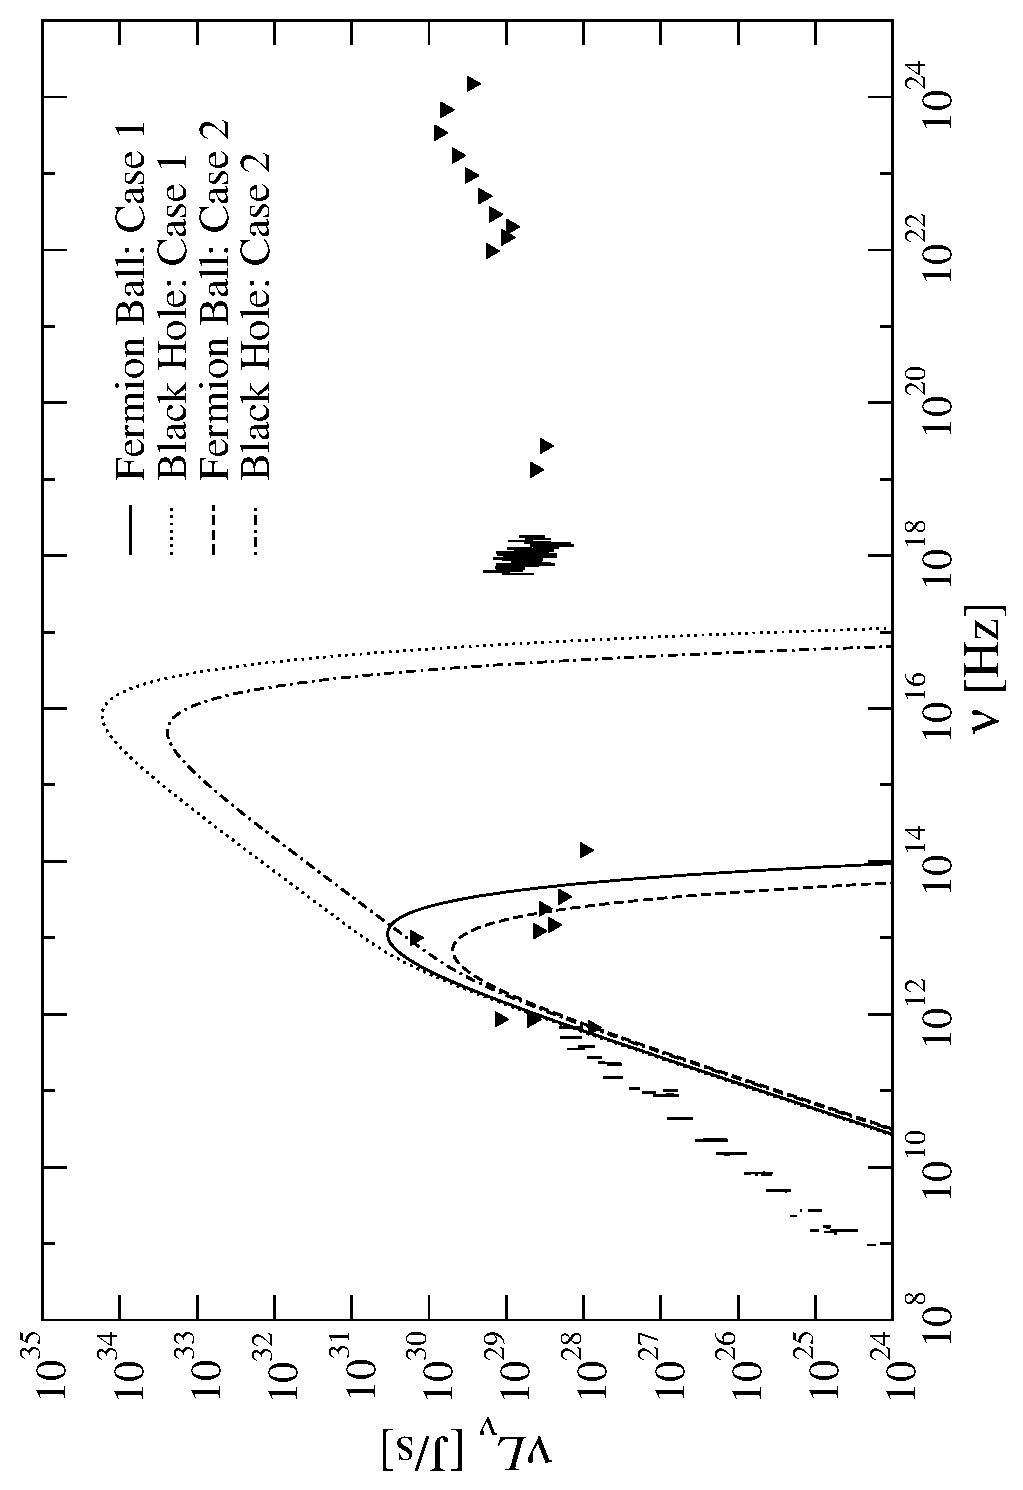
\includegraphics[angle=-90,width=0.9\textwidth]{eps/spectrum-melialimits.eps}
	\caption{The spectrum of the galactic centre due to accretion of gas. ``Case 1'' scenarios have $\dot{M}$=2.948
	$\times 10^{-3}M_\odot$/yr whereas ``Case 2'' scenarios have $\dot{M}$=4.228$\times 10^{-4}M_\odot$/yr.
	Triangular data points are upper limits.}
	\label{fig_accretionspectrummelia}
	\end{center}
\end{figure}

Although the fit from the fermion ball scenario is itself far from perfect, Figure \ref{fig_accretionspectrummelia} clearly shows
that the sudden cut-off in the spectrum around $10^{13}$Hz can indeed be explained by an extended source, and this is the
phenomenon in which we are concerned. The cut-off is due to shearing forces tending to zero at the centre of the fermion ball.
The cut-off can also be explained for the black hole case by using a much lower mass accretion rate.
Unfortunately this will have the consequence that luminosities (at frequencies lower than the cut-off value) are too low. Figure
\ref{fig_accretionspectrumblackholem} displays the spectrum for various mass accretion rates onto a black hole, and Figure
\ref{fig_accretionspectrumfermionballm} the same for the fermion ball scenario.

\begin{figure}[p]
	\begin{center}
	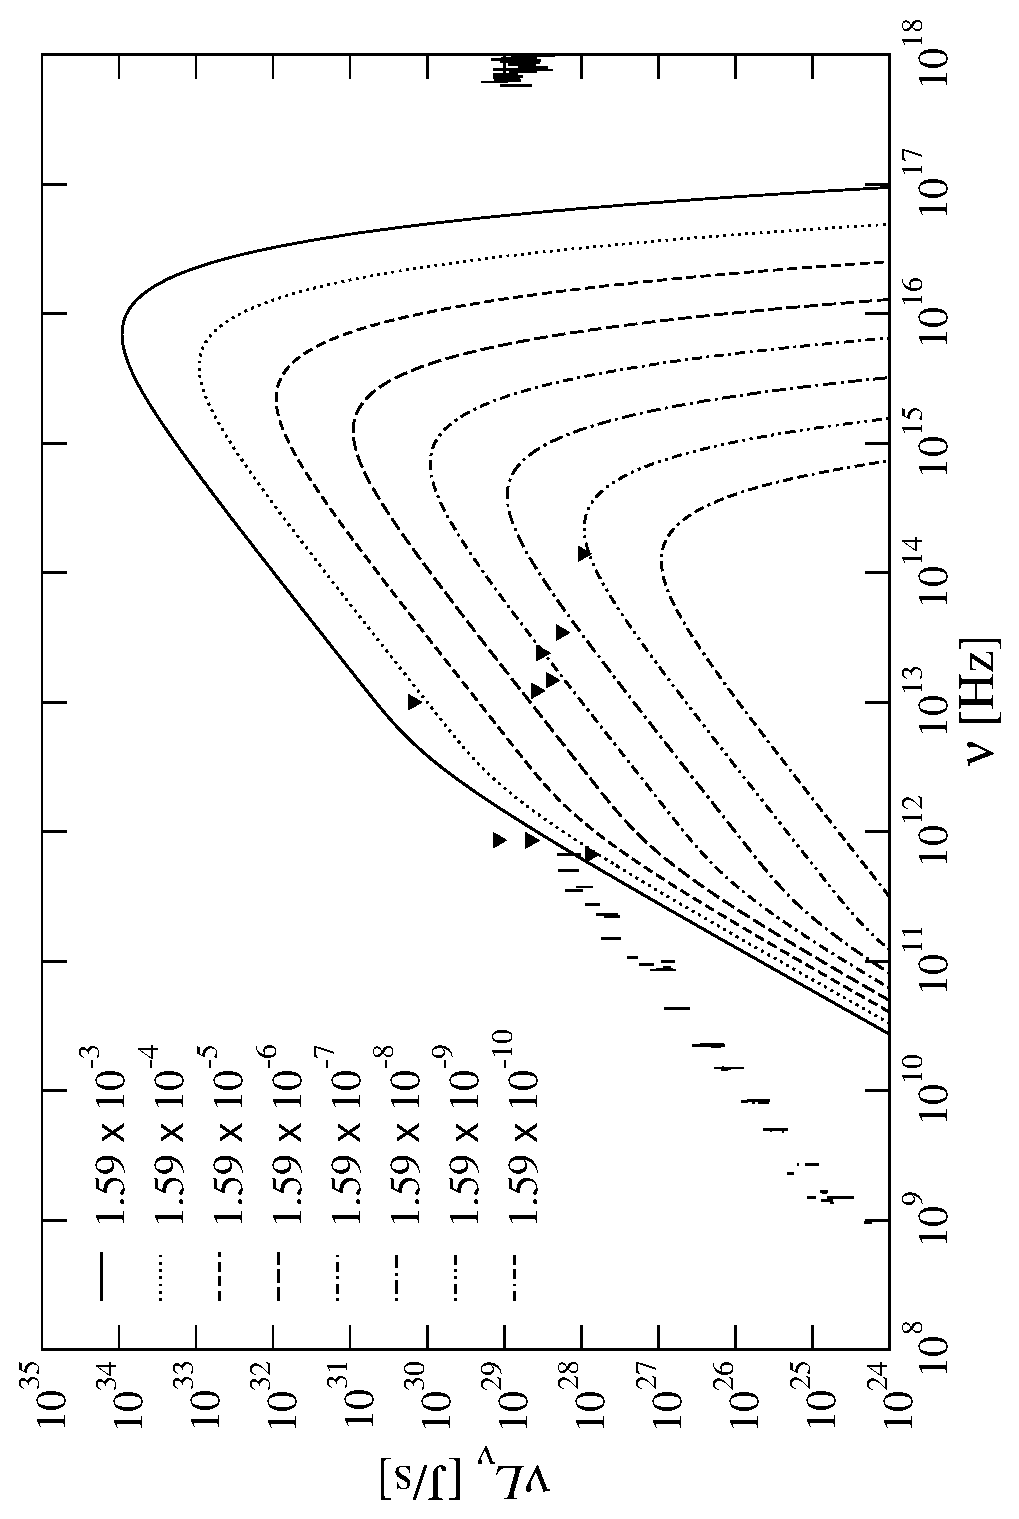
\includegraphics[angle=-90,width=0.9\textwidth]{eps/spectrum-BH-lotsofmdot.eps}
	\caption{The spectrum of the galactic centre due to accretion of gas onto a black hole. Various mass accretion rates are shown in
	units of $M_\odot$/yr.}
	\label{fig_accretionspectrumblackholem}
	\end{center}
\end{figure}
\begin{figure}[p]
	\begin{center}
	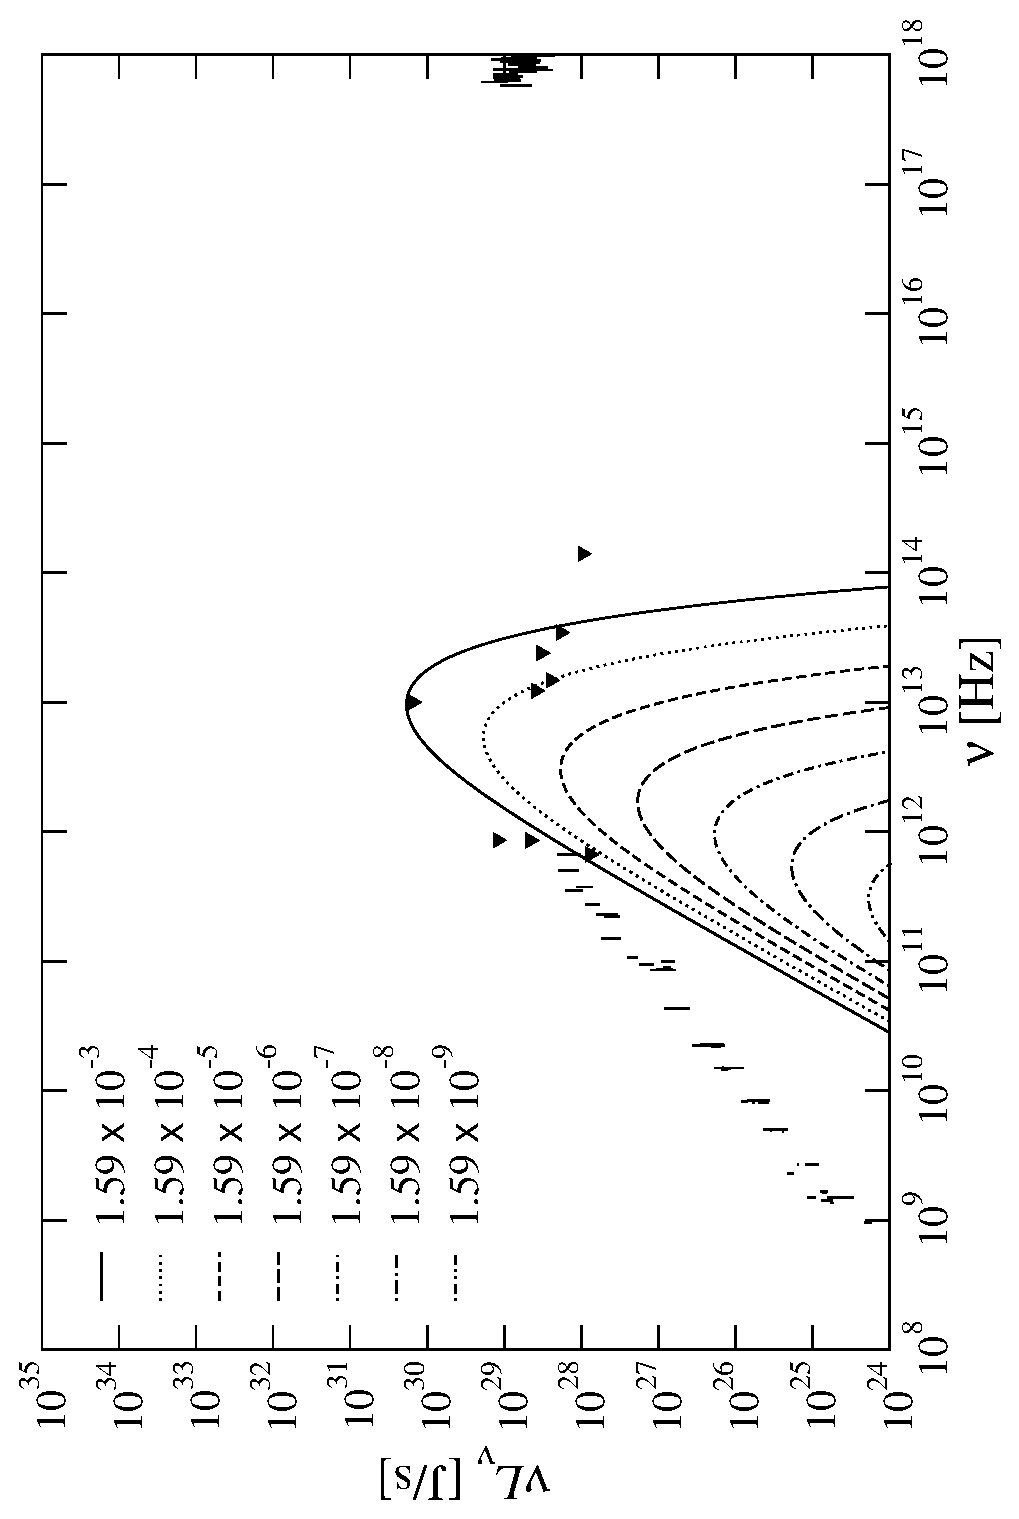
\includegraphics[angle=-90,width=0.9\textwidth]{eps/spectrum-FB-lotsofmdot.eps}
	\caption{The spectrum of the galactic centre due to accretion of gas onto a fermion ball. Various mass accretion rates are shown in
	units of $M_\odot$/yr.}
	\label{fig_accretionspectrumfermionballm}
	\end{center}
\end{figure}

\subsubsection{The Radio and Microwave Spectrum}
Although it has been shown that the fermion ball clearly displays the sudden cut-off in the spectrum in the infra-red region, this simple
model does not explain the `shape' of the spectrum in the radio and microwave region $10^{9} \rightarrow 3 \times 10^{11}$Hz.
Upper limits on the size of the radio source are only a few AU \cite{{ref_radioproper}},
meaning that the emission in this region is not at all due to the
overall accretion of matter, but instead is a result of synchrotron radiation (suggested by the polarisation of the detected photons)
in some localised process. This is evidence of a central object and poses a serious problem to the fermion ball scenario.

\subsubsection{Star Birth}
K-band spectra of stars in the Sgr A* cluster \cite{ref_gezari} reveals that the cluster consists of mainly young, late O $\rightarrow$ early B
main sequence stars. The close proximity of the young stars to the galactic centre is an interesting challenge for either star
formation theory or dynamical theory as the high temperatures, pressures, velocity dispersions and magnetic field strengths in the
central molecular zone inhibit star formation. The black hole scenario is affected even more as there are incredible shearing forces closer
to the nucleus. In the fermion ball scenario the potential becomes harmonic at the centre and shearing forces go linearly to zero, practically
vanishing at $\sim$ 0.01pc.
Using an estimate of new stars simply from the mass accretion rate, a new solar mass star should be expected every 10,000 to 100,000 years
in the fermion ball scenario.
